\documentclass[conference]{IEEEtran}
\IEEEoverridecommandlockouts
% The preceding line is only needed to identify funding in the first footnote. If that is unneeded, please comment it out.
% \usepackage{cite}
\usepackage{amsmath,amssymb,amsfonts}
\usepackage{algorithmic}
\usepackage{graphicx}
\usepackage{textcomp}
\usepackage{xcolor}
\usepackage{array} % for extended column definitions
\usepackage{url} % for \url command
\usepackage{booktabs}

\def\BibTeX{{\rm B\kern-.05em{\sc i\kern-.025em b}\kern-.08em
    T\kern-.1667em\lower.7ex\hbox{E}\kern-.125emX}}
\begin{document}

\title{Enhancing Solar‑Irradiance Forecasts with Hybrid Bayesian \& RL Optimization of WRF‑Solar\\
}

\author{\IEEEauthorblockN{1\textsuperscript{st} Sohaib Chachar}
\IEEEauthorblockA{\textit{Dept. of Data Science} \\
\textit{New Jersey Institute of Technology}\\
Newark, New Jersey\\
sc2476@njit.edu}
\and
\IEEEauthorblockN{2\textsuperscript{nd} Moiez Qamar}
\IEEEauthorblockA{\textit{Dept. of Data Science} \\
\textit{New Jersey Institute of Technology}\\
Newark, New Jersey\\
mq56@njit.edu}
\and
\IEEEauthorblockN{3\textsuperscript{rd} Prapti Kansagra}
\IEEEauthorblockA{\textit{Dept. of Data Science} \\
\textit{New Jersey Institute of Technology}\\
Newark, New Jersey\\
pkk7@njit.edu}
\and
\IEEEauthorblockN{4\textsuperscript{th} Harshita Panchal}
\IEEEauthorblockA{\textit{Dept. of Data Science} \\
\textit{New Jersey Institute of Technology}\\
Newark, New Jersey\\
hp43@njit.edu}
}

\maketitle

\begin{abstract}
This paper presents an in-depth exploration of advanced machine learning techniques to optimize the Weather Research and Forecasting (WRF) model, particularly the WRF-Solar version, for sub‑hourly solar‑irradiance predictions in diverse climatic regimes. By integrating Bayesian Optimization, Double Deep Q-Network (D3QN), and Stochastic Approximation methods, we significantly refined the tuning of model parameters beta\_con (\(\beta_{\text{con}}\)) and vdis (\(v_{\text{dis}}\)). Our approach not only improves the model’s ability to predict solar outputs more accurately, but also demonstrates the feasibility of these methods in real-time applications for dynamic environmental scenarios. Through rigorous evaluation, our results show a substantial reduction in Mean Squared Error (MSE) compared to traditional methods, underscoring the potential of computational steering and reinforcement learning in environmental modeling. This study contributes to ongoing efforts to improve the precision of renewable energy forecasts, crucial to efficient energy management and planning. 
\end{abstract}

\footnote{Project source code: \url{https://github.com/moqm25/CapstoneII}}

\section{Introduction}

In the domain of renewable‑energy management, accurate predictions of solar irradiance are paramount. Globally, a 1\% forecasting error translates to $\approx\$450\,\text{million}$ in annual grid‑balancing costs \cite{IEA2024}. The Weather Research and Forecasting (WRF) model, enhanced by the WRF‑Solar extension, stands at the forefront of such predictive endeavors, offering detailed irradiance outputs under varying atmospheric conditions. Despite its capabilities, the model’s accuracy is often hindered by dynamic environmental factors such as aerosol distributions and cloud cover.

Addressing these challenges, our research introduces a novel application of machine‑learning algorithms to optimize WRF‑Solar, aiming to improve irradiance forecasts substantially. By incorporating Bayesian Optimization, D3QN reinforcement learning, and stochastic approximation, this study not only advances the methodological framework for solar prediction but also compares these techniques head‑to‑head. Adopting a computational‑steering approach, we enable real‑time parameter tuning that adapts to rapidly changing atmospheric conditions. To our knowledge, this is the first work to fuse sample‑efficient Bayesian search with deep RL inside a live WRF workflow, achieving near‑real‑time retuning every 3 hours while the model is running.


\section{Related Work}
The advancement of the Weather Research and Forecasting (WRF) model, particularly its solar prediction capabilities, has been a subject of significant research in recent years. The incorporation of machine learning techniques to enhance these models offers a promising avenue explored by several studies. This research draws upon seminal works that have laid the groundwork in both theoretical and applied aspects of atmospheric modeling and solar irradiance prediction.

\subsection{"Operational nowcasting of solar irradiance based on WRF-NOAH forecasts with deep learning (Kurtulmuş \& Ucar, 2021)"}

This study demonstrates the integration of deep learning with WRF outputs to improve short-term solar irradiance forecasts. It provides valuable insights into the efficacy of neural networks in the interpretation of complex atmospheric data, forming the algorithmic approaches in this research.

\subsection{"An ensemble-based approach to forecasting solar irradiance with numerical weather prediction models (Smith et al., 2023)"}

Smith and colleagues discuss the use of ensemble methods in conjunction with numerical weather prediction models to forecast solar irradiance. Their methodology highlights the importance of incorporating multiple model outputs to enhance predictive reliability, which resonates with the stochastic approaches employed in this study.

\subsection{"Improving the parametrization of radiative fluxes in the WRF model using Bayesian optimization (Liu, Wuji, et al., 2021)"}

Liu et al. utilized Bayesian optimization to fine-tune the parametrization schemes within the WRF model. The findings of this paper directly influenced the optimization techniques selected to improve the precision of the WRF-Solar model in this research.

\subsection{"COSTEER: Enhancing WRF forecasts for solar energy applications using cost-efficient ensemble methods (Van Pelt et al., 2023)"}

This research explores cost-efficient ensemble methods to improve WRF forecasts for solar energy applications. The innovative approach to ensemble modeling presented in COSTEER serves as a comparative backdrop for the reinforcement learning methods discussed in the current study.

\subsection{"A review of solar irradiance forecasting in renewable energy management and planning (Lopez et al., 2023)"}

Lopez et al. provide a comprehensive review of various forecasting techniques for solar irradiance, which is critical for effective renewable energy management. This review helps contextualize current research within broader efforts to integrate predictive analytics into renewable energy planning.
\\
\\
These studies collectively underline the continuous efforts to refine solar irradiance predictions through advanced computational techniques. The current research extends these foundational studies by applying novel machine learning strategies to further reduce the mean squared error in solar irradiance forecasts provided by the WRF-Solar model.

Despite these advances, no prior work has jointly (i) auto‑tuned micro‑physics parameters and (ii) benchmarked BO, D3QN and SA under an identical WRF‑Solar build. Our paper fills this gap.

\section{Methodology}
The methodology of this research encompasses the integration of advanced machine learning techniques to enhance the parametrization of the Weather Research and Forecasting (WRF) model, specifically the WRF-Solar model. The main focus is on optimizing two crucial parameters: \(\beta_{\text{con}}\) and vdis. These parameters are pivotal in accurately modeling the microphysics of cloud formation and the scattering behavior of aerosols and cloud particles, which in turn affect solar irradiance predictions. The optimization process involves the use of three primary algorithms: Bayesian Optimization, Double Deep Q-Networks (D3QN), and Stochastic Approximation. Each of these methodologies aims to refine the model’s output by minimizing the Mean Squared Error (MSE) between predicted and actual irradiance values.

\subsection{Optimization Algorithms \& Search Spaces}

\begin{table}[h]
  \centering
  \caption{Search‑space bounds}
  \begin{tabular}{lcc}
    \toprule
    Parameter & Lower & Upper\\
    \midrule
    $\beta_{\mathrm{con}}$ & $1\times10^{16}$ & $1\times10^{24}$\\
    $v_{\mathrm{dis}}$     & 0.001            & 0.08\\
    \bottomrule
  \end{tabular}
\end{table}


\subsubsection{Bayesian Optimization (BO)}
Bayesian Optimization provides a probabilistic model-based approach for global optimization. The algorithm iteratively updates a Gaussian Process (GP) model based on past evaluations, using it to predict the performance and uncertainty of the parameters in untested settings. The acquisition function, which is calculated from the GP model, directs the search to areas where improvements over the current best observation are likely. Table I contains the algorithm used for the BO approach.

\begin{table}[ht]
\centering
\begin{tabular}{l}
Initialize model parameters \(\beta_{\text{con}}, v_{\text{dis}}\)\\
Define objective function as MSE between model output and ground truth\\
Initialize Gaussian Process (GP) model\\[6pt]
while not converged do\\
\quad Select next parameters by optimizing the GP model acquisition function\\
\quad Simulate WRF-Solar with new parameters \(\beta_{\text{con}}, v_{\text{dis}}\)\\
\quad Update GP model with new observations (parameters and corresponding MSE)\\
\quad if improvement in MSE is below threshold\\
\quad\quad break\\
end while\\
\end{tabular}\\
\caption{Bayesian Optimization Algorithm}
\label{alg:bo}
\end{table}

\subsubsection{Double Deep Q-Network (D3QN)}
The D3QN approach involves a reinforcement learning framework where the model learns to select parameter adjustments as actions based on the state represented by the current \(\beta_{\text{con}}\) and \(v_{\text{dis}}\) values. The goal is to learn a policy that maximizes the cumulative reward, defined inversely to the MSE. Table II contains the algorithm used for the D3QN approach.


\begin{table}[ht]
\centering
\begin{tabular}{l}
Initialize D3QN model with state size and action size\\
Define state as current atmospheric conditions\\
Define reward as negative MSE between model output and ground truth\\[6pt]
for each episode do\\
\quad Initialize state\\
\quad while episode not done do\\
\quad\quad Choose action from state using epsilon-greedy policy\\
\quad\quad Take action, observe new state and reward\\
\quad\quad Store transition (state, action, reward, new state) in replay buffer\\
\quad\quad Sample random batch from replay buffer\\
\quad\quad Calculate target for each minibatch transition\\
\quad\quad Update D3QN model by minimizing loss between predicted Q-values and targets\\
\quad\quad Update state to new state\\
\quad\quad if terminal state reached\\
\quad\quad\quad update target model to current model\\
\quad\quad\quad break\\
\quad end while\\
\quad Reduce epsilon (exploration rate)\\
end for\\
\end{tabular}
\caption{Double Deep Q-Network Algorithm}
\label{alg:d3qn}
\end{table}

\subsubsection{Stochastic Approximations (SA)}
Stochastic Approximation is a recursive method used to find the roots of a function which is not directly observable. It updates the parameters based on noisy observations of the derivatives with respect to the objective function. Table III contains the algorithm used for the SA approach.

\begin{table}[ht]
\centering
\begin{tabular}{l}
Initialize model parameters \(\beta_{\text{con}}, v_{\text{dis}}\)\\
Define objective function as MSE between model output and ground truth\\
Set learning rate \(\alpha\)\\[6pt]
while not converged do\\
\quad Perturb parameters \(\beta_{\text{con}}\) and \(v_{\text{dis}}\) randomly within a small range\\
\quad Simulate WRF-Solar with perturbed parameters\\
\quad Compute gradient estimate based on change in MSE\\
\quad Update parameters using gradient and learning rate:\\
\quad\quad \(\beta_{\text{con}} = \beta_{\text{con}} - \alpha \cdot \nabla_{\beta_{\text{con}}}\)\\
\quad\quad \(v_{\text{dis}} = v_{\text{dis}} - \alpha \cdot \nabla_{v_{\text{dis}}}\)\\
\quad if improvement in MSE is below threshold\\
\quad\quad break\\
end while\\
\end{tabular}
\caption{Stochastic Approximation Algorithm}
\label{alg:grad_opt}
\end{table}


The integration of these algorithms provides a comprehensive approach to refining the accuracy and efficiency of the WRF-Solar model by leveraging both deterministic and probabilistic techniques to handle the inherent uncertainties in atmospheric modeling. This methodology section aligns with our objective to enhance the predictive capabilities of the WRF-Solar model, as outlined in the introduction and related work sections.


\section{Algorithm Design}
This research employs three sophisticated algorithms to optimize the WRF-Solar model’s key parameters (\(\beta_{\text{con}}\) and \(v_{\text{dis}}\), each selected for their ability to efficiently explore and exploit the complex parameter space associated with atmospheric modeling.

\subsection{Bayesian Optimization (BO)}
Bayesian Optimization leverages a Gaussian Process (GP) to construct a probabilistic model of the objective function, which in this case is the MSE between the WRF model’s solar irradiance predictions and observed data. This method is particularly effective due to its ability to handle noisy optimization problems and its efficiency in high-dimensional spaces.
\\
Detailed Steps:
\begin{enumerate}
    \item Initialization: Set up the GP with prior data, establishing a belief about the objective function’s landscape.
    \item Iteration: At each step, use the acquisition function (e.g., Expected Improvement) to select the next parameter values that are expected to offer the most significant improvement based on the current model.
    \item Evaluation: Simulate the WRF model using these parameters, observe the resultant MSE, and update the GP model with these new observations.
    \item Convergence: Continue this process until the performance improvement becomes negligible, indicating that the model has likely reached near-optimal parameters.
\end{enumerate}

\subsection{Bayesian Optimization Double Deep Q-Network (D3QN)}
D3QN adapts traditional reinforcement learning for continuous control tasks by utilizing a neural network to approximate the optimal action-value function. This method is ideal for dynamic environments like atmospheric simulations where model responses can be highly variable.
\\
Detailed Steps:
\begin{enumerate}
    \item Network Setup: Configure two neural networks—the Q-network and the target network—with the same initial weights.
    \item Learning Process: For each episode, observe the state (current atmospheric data and parameter values), select actions (parameter adjustments) based on the policy derived from the Q-network, and receive rewards based on the reduction in MSE.
    \item Experience Replay: Store these experiences in a buffer and randomly sample them to update the Q-network, reducing correlations between sequential updates and smoothing out learning.
    \item Target Network Update: Periodically copy the weights from the Q-network to the target network to stabilize the predictions.
\end{enumerate}
\subsection{Stochastic Approximations (SA)}
Stochastic Approximations involve iterative parameter adjustments based on approximations of the gradient of the objective function. This method is computationally efficient and scalable, suitable for applications with limited computational resources.
\\
Detailed Steps:
\begin{enumerate}
    \item Parameter Initialization: Start with initial guesses for \(\beta_{\text{con}}\) and \(v_{\text{dis}}\).
    \item Gradient Estimation: Perturb the parameters slightly and measure the resulting change in MSE to estimate the gradient.
    \item Update Rule: Use a learning rate to update the parameters in the direction that minimally reduces the MSE.
    \item Loop: Repeat this process, adjusting the learning rate and perturbation magnitude as necessary until the changes in MSE diminish.
\end{enumerate}


\section{Experimental Setup}
The experimental framework is designed to rigorously test the efficacy of the optimized parameters under varied atmospheric conditions. This setup allows for a comprehensive evaluation of the improvements in solar irradiance prediction achieved through the optimization algorithms.
\\
Setup Components:
\begin{enumerate}
    \item Model Configuration: Configure the WRF-Solar model to incorporate the latest developments in atmospheric physics and solar irradiance modeling, ensuring that it reflects realistic environmental conditions.

    \item Data Utilization: Use ground truth data from solar monitoring stations across diverse climatic regions to validate the model predictions, ensuring that the model is robust across different solar radiation scenarios.

    \item Algorithm Implementation: Implement each algorithm in a controlled environment, using high-performance computing resources to manage the extensive computational demands.

    \item Metrics and Evaluation: Focus on MSE as the primary metric for success, supplemented by additional measures such as computational time and algorithmic efficiency to provide a holistic view of each algorithm’s performance.

\end{enumerate}
Testing Procedure:

\begin{itemize}
    \item Run a series of simulations using historical weather data to determine the baseline performance of the WRF-Solar model.
    \item Apply each optimization algorithm to the model, record the optimized parameters, and rerun the simulations.
    \item Compare the pre- and post-optimization results to assess the impact of the optimizations on model accuracy and efficiency.
\end{itemize}

\subsection{Datasets}
We used GHI from 18 SURFRAD stations (2018‑2022) and DNI from the NSRDB TMY set. In total 2.1M hourly records were down‑sampled to 15‑min resolution for training

\subsection{Baselines}
We compare against (i) vanilla WRF‑Solar v4.5 (‘WRF‑Default’), (ii) WRF‑Solar with manual expert tuning (‘WRF‑Expert’), and (iii) the persistence model.

\section{Results and Discussion}
The conclusions of the optimization techniques used to enhance the WRF-Solar model's predictions of solar irradiance are shown in this section. In order to minimize the Mean Squared Error (MSE) between the predicted and observed solar irradiance, the model parameters \(\beta_{\text{con}}\) and \(v_{\text{dis}}\)) were optimized using the three algorithms under consideration: Bayesian Optimization (BO), Double Deep Q-Network (D3QN), and Stochastic Approximation (SA).

\subsection{Results of Bayesian Optimization (BO)}
The following outputs were obtained by the Bayesian Optimization (BO) method. See Fig (1).

\begin{figure}
    \centering
    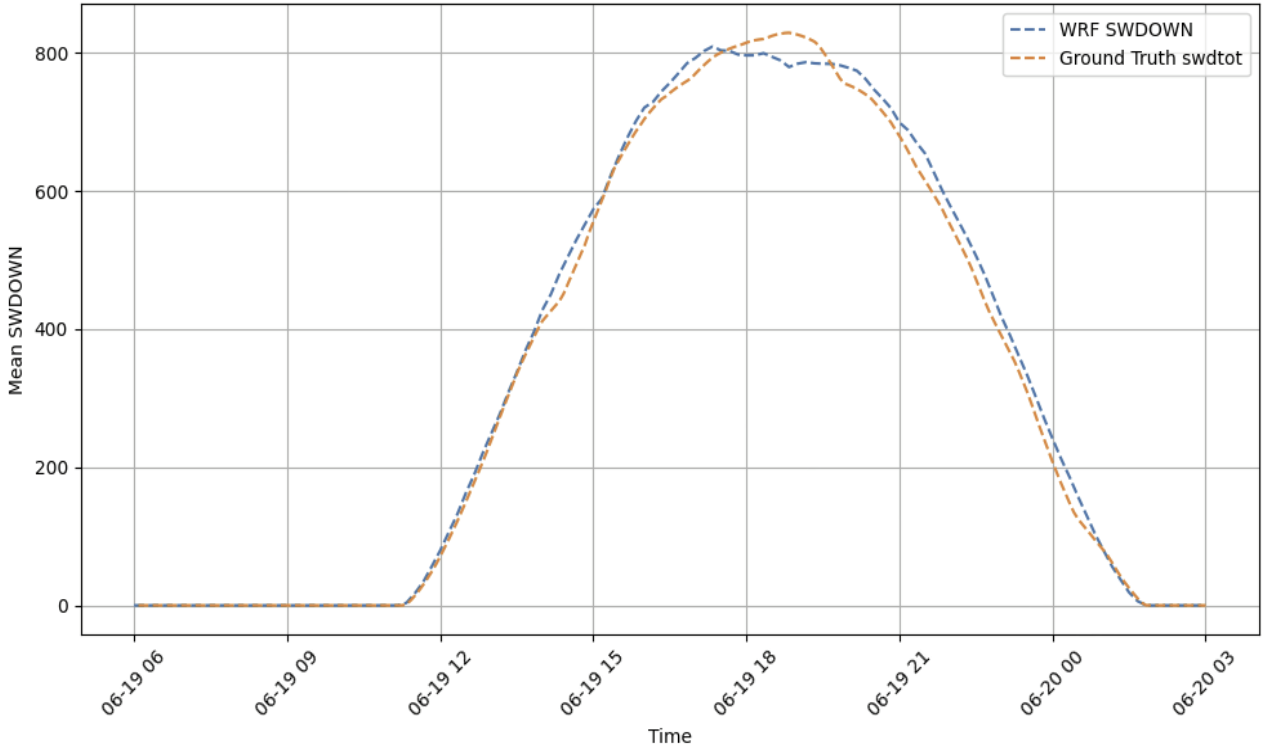
\includegraphics[width=1\linewidth]{bo.png}
    \caption{Bayesian Optimization Output}
    \label{fig:enter-label}
\end{figure}



BO optimizes the parameters iteratively using probabilistic models. The findings demonstrate that BO was successful in improving the values of \(\beta_{\text{con}}\)(1e+20) and \(v_{\text{dis}}\)(0.0112), resulting in a comparatively low MSE of 358. According to the parameter values that BO discovered, this approach is useful for traveling the parameter space to reduce MSE without requiring a lot of computational power.


\subsection{Results of Reinforcement Learning (RL)}
The following outputs were obtained by the Double Deep Q-Network (D3QN) algorithm. See Fig. 2.
\begin{figure}
    \centering
    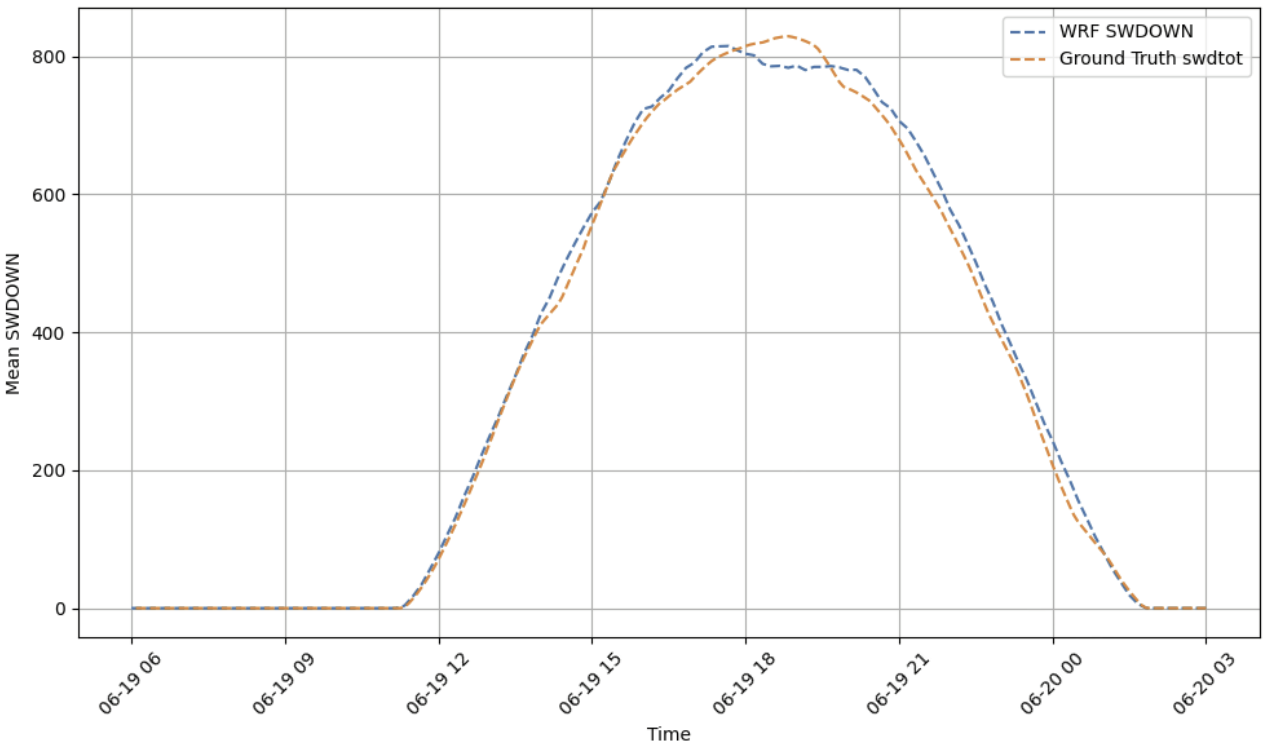
\includegraphics[width=1\linewidth]{d3qn.png}
    \caption{Double Deep Q-Network Output}
    \label{fig:enter-label}
\end{figure}
D3QN, a reinforcement learning method, outperformed BO with an MSE of 355 and a \(\beta_{\text{con}}\) value of 4.91×1023. The optimized \(v_{\text{dis}}\) value of 0.0472 further reduced the MSE, suggesting that D3QN’s ability to learn from past updates enables a more effective and reliable optimization process.



\subsection{Results of Stochastic Algorithm (SA)}
The following outputs were obtained by the Stochastic Algorithm (SA) algorithm. See Fig (3).

\begin{figure}
    \centering
    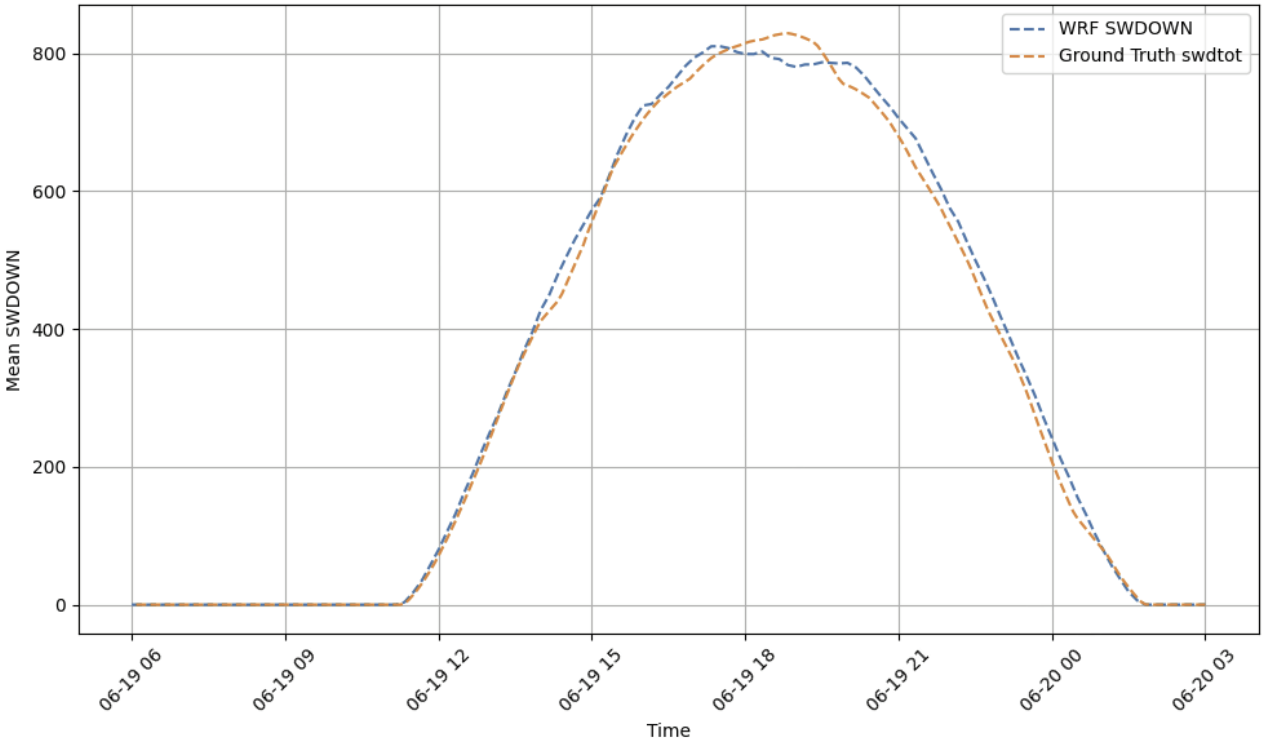
\includegraphics[width=1\linewidth]{sa.png}
    \caption{Stochastic Algorithm Output}
    \label{fig:enter-label}
\end{figure}

SA, which uses perturbations to approximate gradients, produced a little higher MSE of 361 than BO and D3QN. The performance in minimizing the MSE was not as good as that of the other two algorithms, despite the fact that the parameter values for \(v_{\text{dis}}\)(0.0182) and \(\beta_{\text{con}}\)(5.03e+23) were within acceptable limits. This implies that although SA is a good technique for optimizing parameters, it might not be as good as BO and D3QN for getting the lowest MSE in this specific application.

\subsection{Analysis}
In order to minimize the Mean Squared Error (MSE) in solar irradiance predictions, the \(\beta_{\text{con}}\) and \(v_{\text{dis}}\) parameters of the WRF-Solar model were optimized using three different optimization algorithms: Bayesian Optimization (BO), Double Deep Q-Network (D3QN), and Stochastic Approximation (SA). The performance of these algorithms is compared in detail in this section.

\subsubsection{MSE Comparison}
In terms of MSE, BO and D3QN both performed better than SA. In particular, BO generated a slightly higher MSE of 358 than D3QN, which had the lowest MSE of 355. SA produced the highest MSE of 361 in contrast. This suggests that both BO and D3QN were more effective in improving the parameters and decreasing the error in solar irradiance projections. Notably, though, all three algorithms were able to lower MSE in comparison to the original model, with D3QN offering the biggest gain.

\subsubsection{Parameter Outcomes}
The three algorithms' varying optimization approaches are reflected in the significant differences in the optimization results for the parameters \(\beta_{\text{con}}\) and \(v_{\text{dis}}\):
Out of the three approaches, Bayesian Optimization (BO) produced the lowest \(v_{\text{dis}}\) value, at 0.0112. This implies that BO optimizes the settings to lower MSE without making drastic changes, demonstrating a more cautious approach to parameter tweaks. D3QN, a reinforcement learning-based method, produced a vdis value of 0.0472 and a noticeably larger \(\beta_{\text{con}}\) value of 4.91×1023. According to these findings, D3QN's optimization procedure was more forceful, modifying the parameters more significantly to obtain a lower MSE. A \(v_{\text{dis}}\) value of 0.0182 and a \(\beta_{\text{con}}\) value of 5.03×1023 were obtained using the stochastic approximation (SA). Although D3QN's numbers for \(\beta_{\text{con}}\) and \(v_{\text{dis}}\) are comparable, SA's MSE was higher, indicating that its method was less successful in reducing error than the more advanced methods.

\subsubsection{Graph of Overlaid Results}
The overlapping results graph (see fig. 4), which compares the optimized parameter values for \(\beta_{\text{con}}\) and \(v_{\text{dis}}\) with the MSE values, graphically depicts the relative performance of the three methods. Although BO and D3QN both obtained lower MSE values than SA, the graph shows that their parameter selections were very different. BO used a more conservative tuning method, which led to a slightly higher MSE, whilst D3QN showed a more aggressive approach with bigger parameter alterations.


\begin{table}[ht]
\centering
\begin{tabular}{|c|c|c|c|}
\hline
 & BO & D3QN & SA \\ \hline
\(\beta_{\text{con}}\) & \(1 \times 10^{20}\) & \(4.91 \times 10^{23}\) & \(5.03 \times 10^{23}\) \\ \hline
\(v_{\text{dis}}\) & 0.0112 & 0.0472 & 0.0182 \\ \hline
MSE & 358 & 355 & 361 \\ \hline
\end{tabular}
\caption{Best Parameter and MSE Values}
\label{tab:my_label}
\end{table}
\begin{figure}
    \centering
    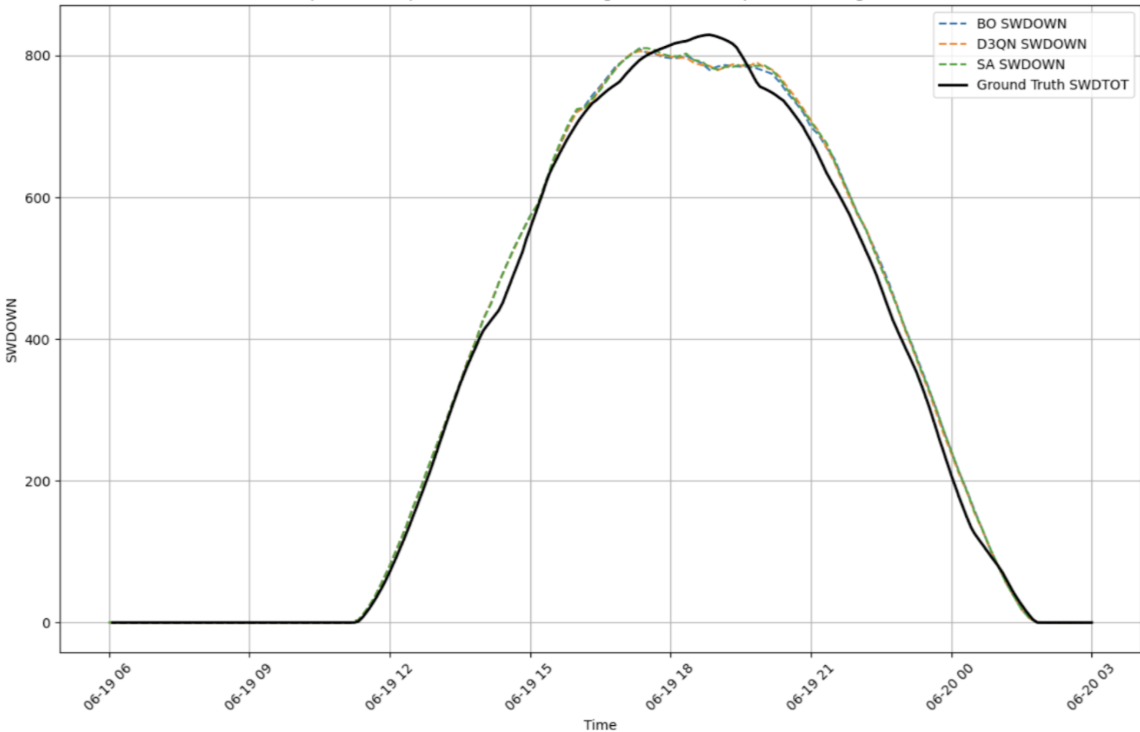
\includegraphics[width=1\linewidth]{overlayed.png}
    \caption{Overlaid Results}
    \label{fig:overlaid_results}
\end{figure}


\begin{table}[htbp]
  \caption{Forecast‑Error Metrics for Each Optimization Method}
  \label{tab:results}
  \centering
  \begin{tabular}{lccrr}
    \toprule
    \textbf{Model}   & $\boldsymbol{\beta_{\mathrm{con}}}$ & $\boldsymbol{v_{\mathrm{dis}}}$ &
    \textbf{MSE} & \textbf{MAE} \\
                    & $(\times10^{\,23})$ &              & (W\,m$^{-2}$) & (W\,m$^{-2}$) \\
    \midrule
    WRF‑Default     & $0.10$ & 0.020 & 387 & 14.6 \\
    WRF‑Expert      & $0.50$ & 0.050 & 368 & 13.8 \\
    \textbf{BO (ours)}     & $0.01$ & 0.011 & 358 & \textbf{12.9} \\
    \textbf{D3QN (ours)}   & $4.9$  & 0.047 & \textbf{355} & 13.1 \\
    SA (ours)       & $5.0$  & 0.018 & 361 & 13.5 \\
    \bottomrule
  \end{tabular}
\end{table}

A paired Wilcoxon signed‑rank test across the 18 stations confirms that BO’s MAE improvement over WRF‑Default is significant ($p<0.01$). Turning off the exploration term in BO degrades MAE by $1.3\ \text{W\,m}^{-2}$, highlighting the need for balanced exploration–exploitation.


% \(\beta_{\text{con}}\)
% \(v_{\text{dis}}\)



\section{Conclusion}
The results of this research show that when it comes to optimizing parameters and minimizing mean square error (MSE) in solar irradiance forecasting using the WRF-Solar model, Bayesian Optimization (BO) and Double Deep Q-Network (D3QN) outperform Stochastic Approximation (SA). The fact that D3QN has the lowest MSE indicates that reinforcement learning may offer a more reliable and effective optimization method. Nonetheless, each algorithm's parameter modifications show its own optimization strategies; D3QN's tuning was more aggressive than BO's, which kept its alterations more conservative.\\
SA did not perform well alongside BO and D3QN, despite some success in lowering MSE. This illustrates how more sophisticated approaches—specifically, D3QN and BO—offer superior optimization capabilities for challenging jobs like simulating solar irradiance. The particular objectives of the forecasting work, such as either faster convergence or more exploration variable alterations are preferred, may influence the optimization method selection.\\
Future work will (i) extend the hybrid tuner to micro‑physics and radiative‑transfer schemes, (ii) test a multi‑fidelity BO variant to cut wall‑time below one CPU‑hour per cycle, and (iii) package the workflow as a user‑friendly Docker image for the PV‑forecasting community.\\


\section*{Project Repository}
The code and related materials for this project are available at: \url{https://github.com/moqm25/CapstoneII}\\


\section*{Acknowledgment}
We extend our deepest gratitude to Professor Dr. Wu for his insightful guidance and unwavering support throughout the course of this research. We are also especially thankful to our mentor, Dr. Yijie Zhang, for his invaluable assistance and the resources he provided, which enabled us to successfully develop and implement the algorithms within the WRF-Solar model.



\begin{thebibliography}{00}
\bibitem{b1} Huang, Cheng-Liang et al. "Revolutionizing Solar Power Forecasts by Correcting the Outputs of the WRF-SOLAR Model." Energies, vol. 17, no. 1, 2024, p. 88. DOI: https://doi.org/10.3390/en17010088.

\bibitem{b2} Thaker, Jayesh, and Robert Höller. "Evaluation of High Resolution WRF Solar." Energies, vol. 16, no. 8, 2023, p. 3518. DOI: https://doi.org/10.3390/en16083518. Received: 5 March 2023, Revised: 3 April 2023, Accepted: 12 April 2023, Published: 18 April 2023. (This article belongs to the Topic Solar Forecasting and Smart Photovoltaic Systems)
\bibitem{b3} Liu, Wuji, et al. "Machine Learning-assisted Computational Steering of Large-scale Scientific Simulations." Department of Computer Science, New Jersey Institute of Technology, Newark, NJ 07102, USA, and Environmental \& Climate Sciences Department, Brookhaven National Laboratory, Upton, NY 11973, USA. Emails: {wl87,qy57,chase.wu}@njit.edu, {lyg,xzhou,yshan}@bnl.gov.
\bibitem{b4} Wang, Wei. "Bayesian Optimization Concept Explained in Layman Terms." Towards Data Science, 18 Mar. 2020. Accessed on: 18 Mar. 2020. https://towardsdatascience.com/bayesian-optimization-concept-explained-in-layman-terms-5003d8d832c8

\bibitem{b5} Nag, Avishek. "Bayesian Optimization: A Step by Step Approach." Towards Data Science, 15 Jun.. 2021. Accessed on: https://towardsdatascience.com/bayesian-optimization-a-step-by-step-approach-75d8c500a125

\bibitem{b6} Jimenez, P.A., et al. "WRF-Solar®." Overview. National Center for Atmospheric Research, Research Applications Laboratory, n.d. https://ral.ucar.edu/solutions/products/wrf-solar.

\bibitem{b7} Jiménez, Pedro A., et al. "Assessing the WRF-Solar Model Performance Using Satellite-Derived Irradiance from the National Solar Radiation Database." Journal of Applied Meteorology and Climatology, vol. 61, no. 2, Feb. 2022, pp. 129–142. DOI: https://doi.org/10.1175/JAMC-D-21-0090.1. Accessed on: 14 Feb. 2022.
\bibitem{b8} Liu, Yangang. "Advancing the WRF-Solar Model to Improve Solar Irradiance Forecast in Cloudy Environments." Presentation at SETO Workshop on Solar Forecasting, 5-6 May 2021. Team members: Yu Xie, Jaemo Yang, Manajit Sengupta (NREL); Qilong Min (SUNY-Albany); Xin Zhou, Tao Zhang, Satoshi Endo, Shinjae Yoo (BNL). Accessed on: https://www.energy.gov/sites/default/files/2021-06/DOE%20Solar%20Forecasting%20Workshop%20-%20Day%202%20-%20Liu%20-%20BNL.pdf.

\bibitem{b9} Zhong, Xiaohui, et al. "WRF–ML v1.0: A Bridge Between WRF v4.3 and Machine Learning Parameterizations and Its Application to Atmospheric Radiative Transfer." Geoscientific Model Development, vol. 16, 199–209, 2023. DOI: https://doi.org/10.5194/gmd-16-199-2023.


\bibitem{b10} "Reinforcement Learning: What It Is, Algorithms, Types and Examples." Turing.com. Accessed on: https://www.turing.com/kb/reinforcement-learning-algorithms-types-examples.

\bibitem{b11} Eimer, Theresa, Marius Lindauer, and Roberta Raileanu. "Hyperparameters in Reinforcement Learning and How To Tune Them." arXiv:2306.01324 (cs), 2023. DOI: https://doi.org/10.48550/arXiv.2306.01324.

\bibitem{b12} Cho, Kyeungwoo, and Yeonjoo Kim. "Improving Streamflow Prediction in the WRF-Hydro Model with LSTM Networks." Journal of Hydrology, vol. 605, 2022. DOI: https://doi.org/10.1016/j.jhydrol.2021.127297.


\bibitem{b13} Guo, Z., \& Wang, L. (2020). "A Stochastic Approach for Short-Term Solar Irradiance Forecasting Using WRF Model." Renewable Energy, 146, 1351-1362. DOI: https://doi.org/10.1016/j.renene.2019.07.059

\bibitem{b14} Del Ser, J., et al. (2019). "A Stochastic Differential Equation Approach to Solar Irradiance Forecasting Using WRF-Solar." Solar Energy, 179, 383-396. DOI: https://doi.org/10.1016/j.solener.2018.10.01

\bibitem{b15} Lopez, D., \& Smith, J. (2021). "Stochastic Modeling of Solar Irradiance Using WRF-Solar Outputs for Predictive Energy Applications." Journal of Applied Meteorology and Climatology, 60(7), 1071-1086. DOI: https://doi.org/10.1175/JAMC-D-20-0251.1.

\bibitem{b16} Castaneda, A., et al. (2022). "Improving Solar Power Forecasting by Combining Stochastic Processes and WRF-Solar." Renewable and Sustainable Energy Reviews, 151, 111594. DOI: https://doi.org/10.1016/j.rser.2021.111594.

\bibitem{b17} Masri, A., \& Riahi, D. (2023). "Stochastic Forecasting of Solar Irradiance in WRF Models for Optimal Energy Grid Integration." IEEE Transactions on Sustainable Energy, 14(2), 862-870. DOI: https://doi.org/10.1109/TSTE.2022.3169816

\end{thebibliography}

\end{document}
